\documentclass{article}

\usepackage{fullpage}
\usepackage{amsfonts, amsmath}
\usepackage{url}
\usepackage{hyperref}
\usepackage[xindy, toc]{glossaries}
\usepackage{graphicx}
\usepackage[final]{pdfpages}

\pagenumbering{gobble}

\hypersetup{
    colorlinks=true,
    linkcolor=black
}

\makeglossaries

\begin{document}
\clearpage
\vspace*{\stretch{2}}
\begin{center}
\begin{minipage}{.6\textwidth}

\title{Automatic Music Generator \\ \vspace{2 pt} \Large{Project Proposal}}
\author{Sam Fleckenstein (sef44)\\*Ross Nanopoulos (rdn21)}
\date{February 7, 2014}
\maketitle

\end{minipage}
\end{center}
\vspace{\stretch{3}}
\clearpage

\tableofcontents
\newpage

\newglossaryentry{name=time signature,description=notational convention to specify how many beats are in each measure.}
\newglossaryentry{name=tempo,description=the speed or pace of a given piece and derives directly from the average beat duration.}
\newglossaryentry{name=segment,description=a set of sound entities (typically under a second), relatively uniform in timbre and harmony.}
\newglossaryentry{name=tatums,description=are subdivisions of beats}
\newglossaryentry{name=beats,description=are subdivisions of bars}
\newglossaryentry{name=bars,description=a segment of time defined as a given number of beats; bar offsets also indicate downbeats, the first beat of a measure.}
\newglossaryentry{name=sections,description=defined by large variations in rhythm or timbre (e.g. chorus, verse, bridge, guitar solo, etc.)}
\newglossaryentry{name=key,description=is a track-level attribute ranging from 0 to 11 and corresponds to one of the 12 keys: C, C#, D, etc. up to B.}
\newglossaryentry{name=mode,description=is equal to 0 or 1 for minor or major, respectively, and may be -1 in case of no result}
\newglossaryentry{name=loudness,description=given by three data points: dB value at onset, dB value at peak, and a segment-relative offset for peak loudness}
\newglossaryentry{name=pitch,description=given by normalized vector corresponding to the 12 pitch classes with values from 0 to 1. Noisy sounds represented by values close to 1; pure tones described by one value at 1 (the pitch) and others near 0.}
\newglossaryentry{name=timbre,description=the quality of the musical note or sound that distinguishes different types of musical instruments or voices.}
\newglossaryentry{name=audio fingerprint,description=a condensed digital summary, deterministically generated from an audio signal that can be used to identify an audio sample or quickly locate similar items in an audio database.}


\printglossary[title=Terms and Abbreviations,toctile=Terms and Abbreviations]
\newpage

\section{Abstract}
The purpose of this project is to develop an intelligent music composer that will analyze common and popular patterns in music, reason about those patterns, and generate a new piece of music that is significantly different than the analyzed pieces, while still being interesting.

\section{Background}
What is the process by which humans make music? They study the fundamentals: beats, measures, time and key signatures, tempo, rhythm. They listen to great composers: Bach, Tchaichovsky, Mahler, Debussy, Chopin. Somehow this knowledge combined with creativity yields additional, masterful compositions. How then, does one enable a computer to exhibit this thoughtful creativity?\\
\\
A variety of methods have been proposed for algorithmic composition including hidden Markov models \cite{5492670}, genetic algorithms \cite{514161}, and neural networks \cite{4667040}. Additionally, a field known as "combination theory" has combined these methods to create more advanced learning and composition algorithms \cite{4626654}. Hidden Markov Models utilize an element of probability and uncertainty that can lead to much more interesting compositions
\cite{5492670}, which is the primary method of algorithmic composition that the system in this report will use.\\
\\
The argument can be made that innate creativity plays a large role in being able to compose interesting music.  However, the goal of artificial intelligence is to eventually develop systems that can think and have personalities of their own.  Thus, this innate creativity when composing music will come with more advanced artificially intelligent systems that can think for themselves and exhibit such behavior.

\section{Intended Audience}
Researchers who would like to incorporate different learning techniques for algorithmic composition will be able to easily integrate with this system. Additionally, it will be easy enough to use for someone who has no musical talent, but still wants to compose music.

\section{Architecture Design}
\subsection{Song Parser}
The backbone of the song parser will be The Echo Nest's large database of music intelligence. The song parser will utilize The Echo Nest's API to extract useful song information from the database, which includes a plethora of aspects including time signature, key, mode, tempo, loudness, duration, end of fade in, start of fade out, audio fingerprint, timbre, pitch, and loudness. Additionally, The Echo Nest provides sequenced data as "musically relevant elements" that include segments, tatums, beats, bars, and sections. This information will allow the learning agent to discern the myriad dynamics of songs and learn about the ways in which different songs are composed.

\subsection{Learning Agent}
The job of the learning agent will be to take the raw music data gathered by Echo Nest and discover the relevant patterns in the music. There are a number of different algorithms that could be used to achieve this goal, but this project use a hidden Markov model to extract these patterns. This model was chosen because it can be used to represent processes where not all of the information about a state is known. This is useful because music is very complex and it is very difficult to determine every variable that goes into determining what should come next in a song. Another reason that hidden Markov models were chosen for this project is because they have been successfully applied the automatic generation of music \cite{5492670}. The complexity of a hidden Markov model is also very easy to expand. This can be done by looking at data that is farther in the past from the current observation, or by adding in more variables to the states you are considering \cite{Wiki}.\\

\subsection{Composition Agent}
The composition agent will take the information that the learning agent provides and decide which notes, patterns, rhythms, etc. to incorporate into its own piece of music. It will then be responsible for outputting this generated music to a .wav file, which can be used later for further analysis.

\section{Project Management}
Below is a Gantt Chart, which will drive our development process and schedule:
\begin{figure}[ht]
\center{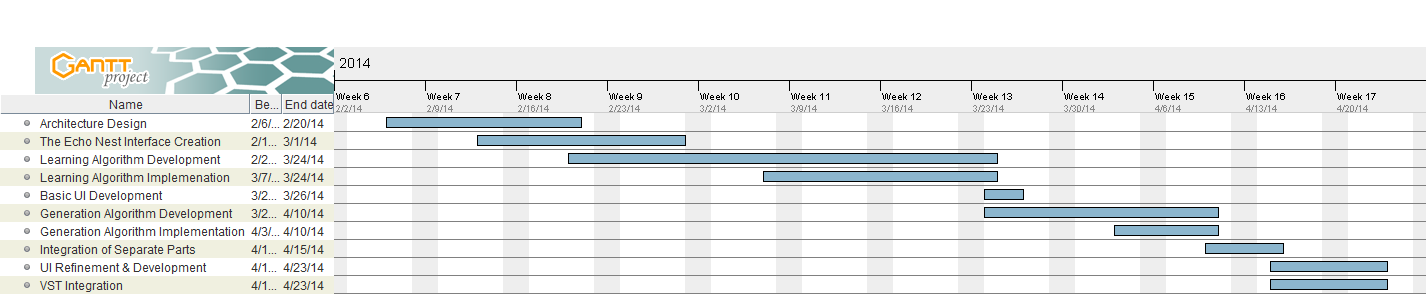
\includegraphics[width=\linewidth]{gantt.png}}
\end{figure}
These dates were decided by the best estimate of how long each component will take to implement.  The development of the learning and composition algorithms will take the most time and will be in continuous development; therefore, they overlap with many other aspects of the project.  The user interface will take less time to implement, and can be incorporated into other stages of development.  Additional features such as VST support will be completed towards the end of the project as time permits.

\subsection{Communication}
In order to facilitate on-time delivery of the Intelligent Music Generator, in-person meetings will be held at least once at week on Thursdays at 4:30. In addition to this, meetings will be held as necessary to discuss upcoming deadlines as well as any issues that have come up. Communication will also happen during the rest of the week primarily via email.

\subsection{Source Control}
Github will be used for feature tracking and reporting bugs.  Pull requests will be utilized to ensure that each member has reviewed the code before it enters the master branch.  Branches will be utilized for implementing different components and features.

\subsection{Work Division}
The primary responsibilities of each of the project members are as follows. Sam will be responsible for the primary development and implementation of the learning algorithms. Ross will be in charge of the interface to The Echo Nest's API, as well as the development and implementation of the composition algorithms. This is not a hard division of the work as each of the group members will also be working a great deal on the parts of the project they are not in charge of. This division of work fits well with the strengths and experience of each of the project members.

\section{Completed Work}
The work that is completed so far has been mostly research based. Various learning techniques for the learning agent have been examined before settling on using a Hidden Markov model. This model was chosen for several reasons. First, because it has been applied to various other projects with similar goals to this one \cite{761266, 1394661} . Second, because it appears to be complex enough to produce interesting music, but simple enough that it will be possible to complete the project in the given timeline.\\

\section{Software Requirements}
\subsection{The Echo Nest Interface}

\subsubsection{The Echo Nest API}
The Echo Nest API allows a user to search their catalog by a variety of methods that respond in JSON or XML, but only the JSON responses will be used.  Many of the attributes in the JSON responses have confidence levels down to the beat, which is the Echo Nest's confidence of how likely the logical beat represents a real physical beat in the song.

\subsubsection{Interface Component}
This component will interact with The Echo Nest's API and database. It will make a call using the API determined by user input. It will be fed a seed note, chord, key, or other attributes from which the parser can locate and return relevant songs. For example, the song parser could be passed in a genre of rock, with a seed note of "A", a time signature of 4/4, and a tempo of 180-200 beats per minute. This will allow the calls to The Echo Nest's API to be more specific, so that the other parts of the automatic music generator will have more specific data with which to reason. The Echo Nest's API returns JSON objects that can be passed on by the song parser, in order to be used by the learning agent in its reasoning.

\subsection{Learning Agent}
\subsubsection{Internal Architecture}
The learning agent will use the GHMM library \cite{GHMM} to perform the required machine learning. This library was chosen because it offers all of the features needed to perform the required learning task. It is also free, another important feature.

\subsubsection{Parser to Learning Agent Interface}
In order to make the learning agent as modular as possible, the interface between it and the song parser will be kept very small, and will consist of a single call to the parser to get the raw song data. This will make it easier to swap out the learning algorithm if the need arises.

\subsubsection{Learning Agent to Composition Agent Interface}
Similar to the interface between the parser and the learning agent, this interface between the learning agent and the composition agent will be kept as small as possible. The only interaction between these two components will be when the learning agent passes the composition agent a file containing a representation of all of the relevant patterns that it found in the music.

\subsection{Composition Agent}
The composition agent will take the relevant patterns provided by the learning agent and decide which patterns should be utilized in its composition. It will consist of an algorithm to decide which of the relevant patterns will be chosen, as well as a component to write a .wav file to disk.  Additionally, there will be a component to compare the new song with the songs that were used to create it.

\section{Software Specifications}
\subsection{UI}
\begin{enumerate}
\item The UI will prompt the user for a musical genre
\item The UI will prompt the user for a song tempo
\item The UI will prompt the user for a time signature
\item The UI will prompt the user for a key signature
\item The UI will send these user choices to the Echo Nest Interface
\end{enumerate}

\subsection{The Echo Nest Interface}
\begin{enumerate}
\item The Echo Nest Interface will take as input the user input from the UI
\item The Echo Nest Interface will make a call to The Echo Nest API using the user input
\item The Echo Nest will output JSON objects to the Learning Agent
\end{enumerate}

\subsection{Learning Agent}
\begin{enumerate}
\item The learning agent will use the GHMM library
\item The learning agent will take as input JSON objects from the Echo Nest Interface
\item The learning agent will train a model \cite{GHMM} using the GHMM library and the input from the Echo Nest Interface
\item The learning agent will output a trained model to the composition agent
\end{enumerate}

\subsection{Composition Agent}
\begin{enumerate}
\item The composition agent will take as input a trained model from the learning agent
\item The composition agent will create an overarching chord progression
\item The composition agent will then fill in notes using the trained model
\item The composition agent will write the resulting composition to disk as a .wav file
\end{enumerate}

\subsection{User Feedback}
\begin{enumerate}
\item The user will be prompted to rate a number of short song clips
\item The user ratings will be tabulated and used to update the learned model based on which musical patterns the user rated highest
\item The user will be presented with one longer song based on the updated musical model
\end{enumerate}

\section{Wishlist Features}
Another feature that may be added is a different learning algorithm. If there is time, neural networks or genetic algorithms may be explored and added to do the learning, instead of just using a hidden Markov model.\\
\\
A third feature that will be added if there is time is the ability to output the music to a Virtual Studio Technology. This would allow songs to be created that have more than one instrument. It would also allow the user or program to select what instrument they would like to use.

\section{Project Challenges}
\subsection{User Feedback}
One of the main challenges with this project will be incorporating user feedback in some meaningful way. It would not be terribly difficult to write a program that produces some kind of music, but to write a program that successfully uses user feedback to improve the music created is much more challenging. It is also challenging to get useful data from a user who is asked to rate an entire song without having the user rate thousands of different songs. To address these challenges, the system will ask the user to rate short snippets of music that represent key patterns in the training data (i.e. the most common patterns from that music). These ratings will be used to determine which patterns the user likes the most, which will then be reflected in an update to the trained music model.

\subsection{Extracting Patterns}
The process of extracting the patterns that define a user specified set of music will be very challenging. To address this challenge, the task of learning has been simplified as much as possible. This has been done by choosing to use an already created hidden Markov model learning library that fits the needs of this project, rather than implementing an entirely new learning algorithm

\nocite{*}

\bibliography{References}
\bibliographystyle{plain}

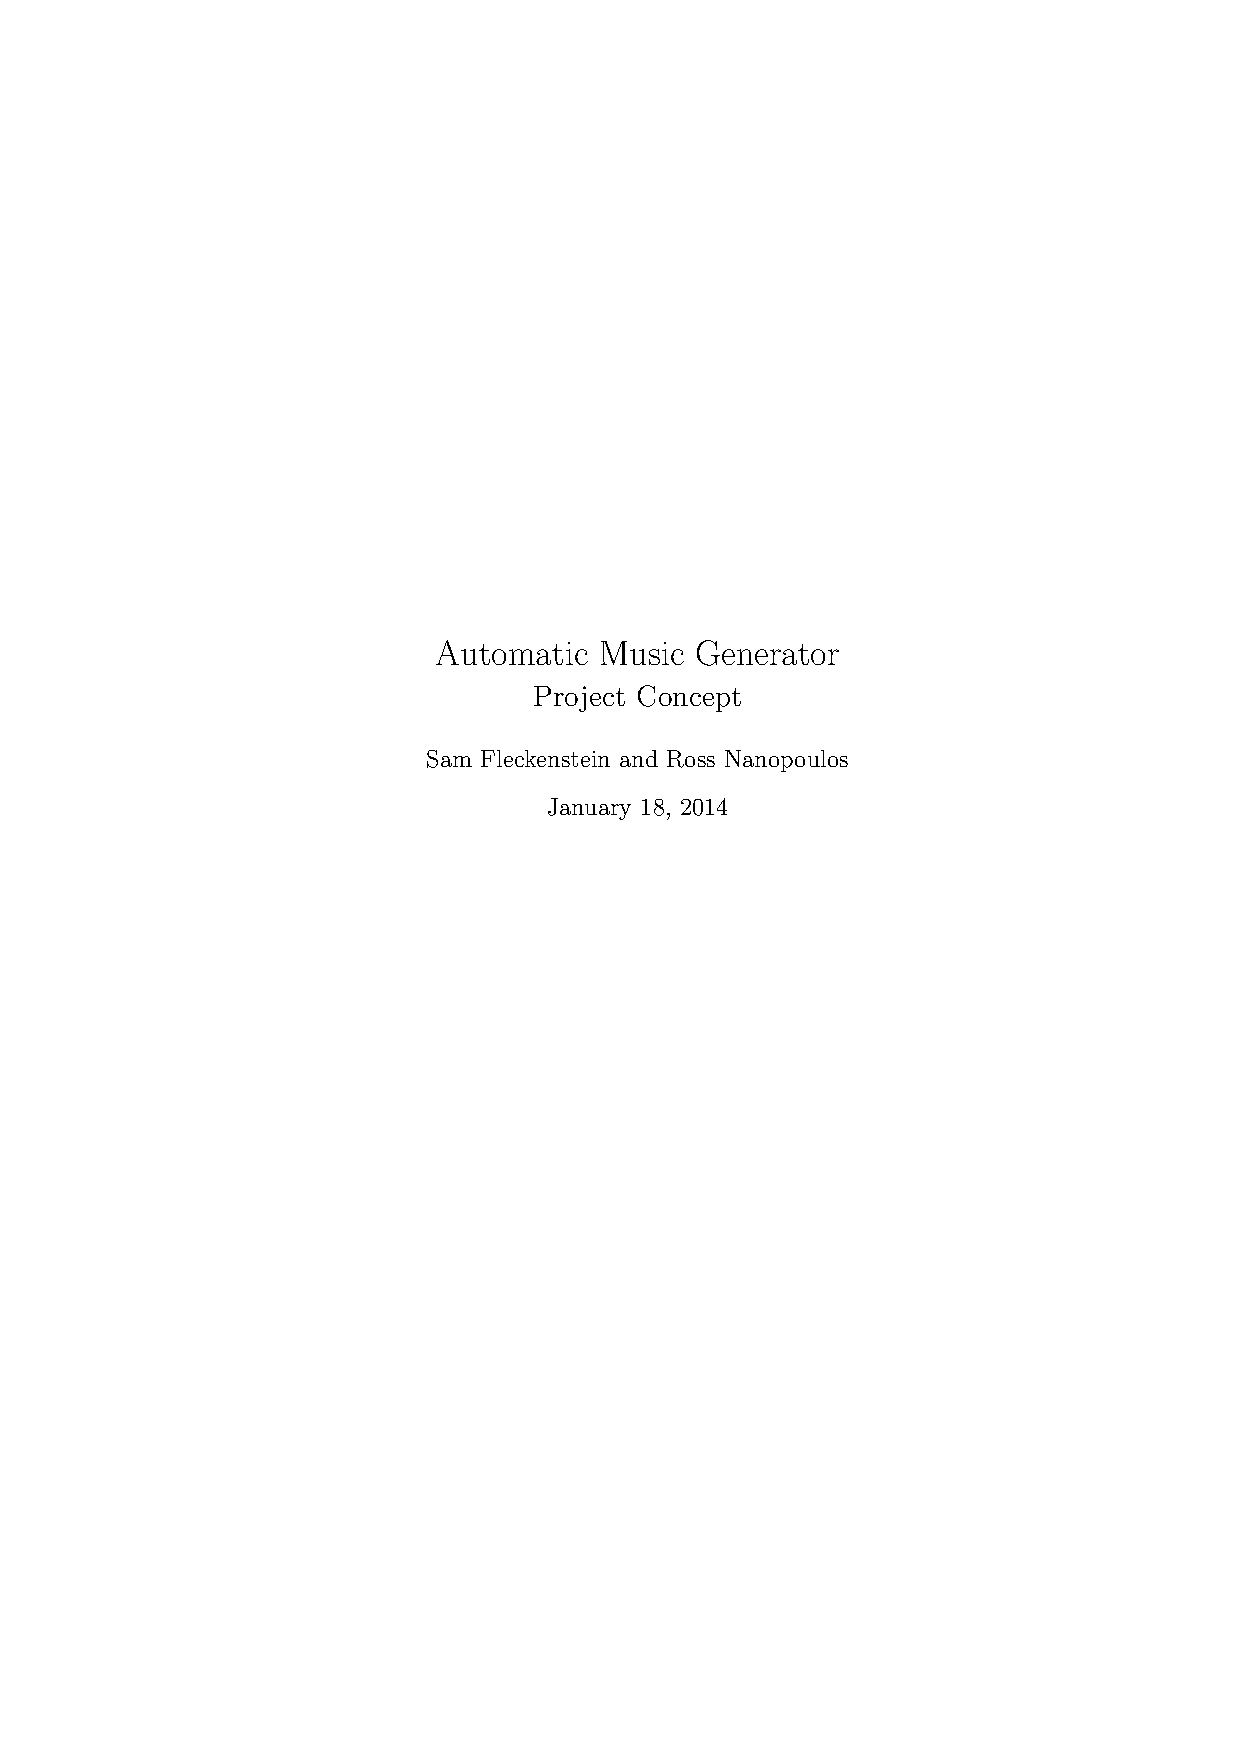
\includepdf[pages=-]{Concept.pdf}

\end{document}
